%Sprawozdanie z Fiz3.1 Jan Bronicki
\documentclass{article}
\usepackage[utf8]{inputenc}
\usepackage{graphicx}
\graphicspath{ {graph1.png},{graph2.png} }
\usepackage[margin=2.5cm]{geometry}
\usepackage{array}
\usepackage{wrapfig}
\usepackage{multirow}
\usepackage{tabularx}
\usepackage{amsmath}
\usepackage{mathtools}
\usepackage[table]{xcolor}
\usepackage{multirow}
\usepackage{polski}
\title{Sprawozdanie 1}

\author{Jan Bronicki \\
Nr indeksu: 249011\\
Ćwiczenie: 100b}
\date{}
\begin{document}

\maketitle


%---------------------------------------------------------------------

\begin{center}
    \renewcommand{\arraystretch}{1.3}
\begin{tabular}{ |c|c|c|c|c|c|c|c|c|c| }
    \hline
    U(V)&u(U)[V]&I[mA]&u(I)[mA]&R[$\Omega$]&$u_c(R)[\Omega]$&$\bar{R}[\Omega]$&$u(\bar{R})[\Omega]$&$R_w[\Omega]$&$u_c(R_w)[\Omega]$ \\
    \hline \hline
    3.29&$\pm$0.02&18.7&$\pm$0.2&175.94&$\pm$ 2.16& \multirow{6}{*}{175}&\multirow{6}{*}{$\pm$0.62}&\multirow{6}{*}{175.75}&\\ 
    \cline{1-6}

    4.78&$\pm$0.02&27.8&$\pm$0.3&171.94&$\pm$ 1.99&&&&\\ 
    \cline{1-6}
  
    6.35&$\pm$0.02&36.1&$\pm$0.3&175.90&$\pm$ 1.70&&&&\\ 
    \cline{1-6}

    7.89&$\pm$0.03&44.9&$\pm$0.4&175.72&$\pm$ 1.41&&&&\\ 
    \cline{1-6}

    9.50&$\pm$0.03&54.2&$\pm$0.4&175.28&$\pm$ 1.51&&&&\\ 
    \cline{1-6}
    
    12.44&$\pm$0.04&71.0&$\pm$0.6&175.21&$\pm$ 1.58&&&&\\ 
    \hline
\end{tabular}
\label{tabular: t}
\end{center}
%---------------------------------------------------------------------
Przykładowe obliczenia:
\begin{center}
    Delta niepewności napięcia:\\*
    $\Delta u(U)  = 0.5\% \cdot rdg+1 \cdot dgt=\cfrac{0.5}{100} \cdot 3.29 + 0.01=0.0264\approx0.03$\\*
    Niepewność napięcia:\\*
    $u(U)=\cfrac{\Delta u(U)}{\sqrt{3}}=0.015\approx0.02$\\*
    Delta niepewności natężenia:\\* 
    $\Delta u(I) = 1.2\% \cdot rdg+1 \cdot dgt = \cfrac{1.2}{100} \cdot 18.7 +0.1 =0.3244$\\*
    Niepewność natężenia:\\*
    $u(I)= \cfrac{\Delta u(I)}{\sqrt{3}} \approx 0.2$\\*
    Opór:\\* 
    $R=\cfrac{U}{I} = \cfrac{3.29}{0.0187} \approx 175.94 \ \Omega$\\*
    %%%%%%%%%%%%%%%
    Niepewność całkowita R:\\*
    $u_c (R)=\sqrt{\sum_{j=1}^{k}\left( \cfrac{\partial f}{\partial x_j}\right)^2 u^2 (x_j)}
    =\sqrt{\cfrac{u^2 (U)}{I^2} + \cfrac{U^2 \cdot u^2 (I)}{I^4}}=$
    $= \sqrt{\cfrac{\left(\cfrac{0.02}{1000}\right)^2}{0.0187^2} + \cfrac{3.29^2 \cdot \left(\cfrac{0.2}{1000}\right)^2}{0.0187^4}}\approx 2.16$\\* 
    %%%%%%%%%%%%%%%
    Wartość średnia R:\\* 
    $\bar{R} = \cfrac{\sum_{i=1}^{n}x_i}{n}=174.9983333 \approx 175\Omega$\\*
    Niepewność wartości średniej R:\\ *
    $u(\bar{R}) = \sqrt{\cfrac{\sum_{i=1}^{n} \left(x_i - \bar{x} \right)^2}{n(n-1)}}\approx 0.62$\\*
    Opór wewnętrzny:\\* 
    $R_w =\cfrac{1}{A}=\cfrac{1}{0.00569} \approx 175.75 \ \Omega$\\*

\end{center}
\newpage
\begin{figure}[h]
    \centering
    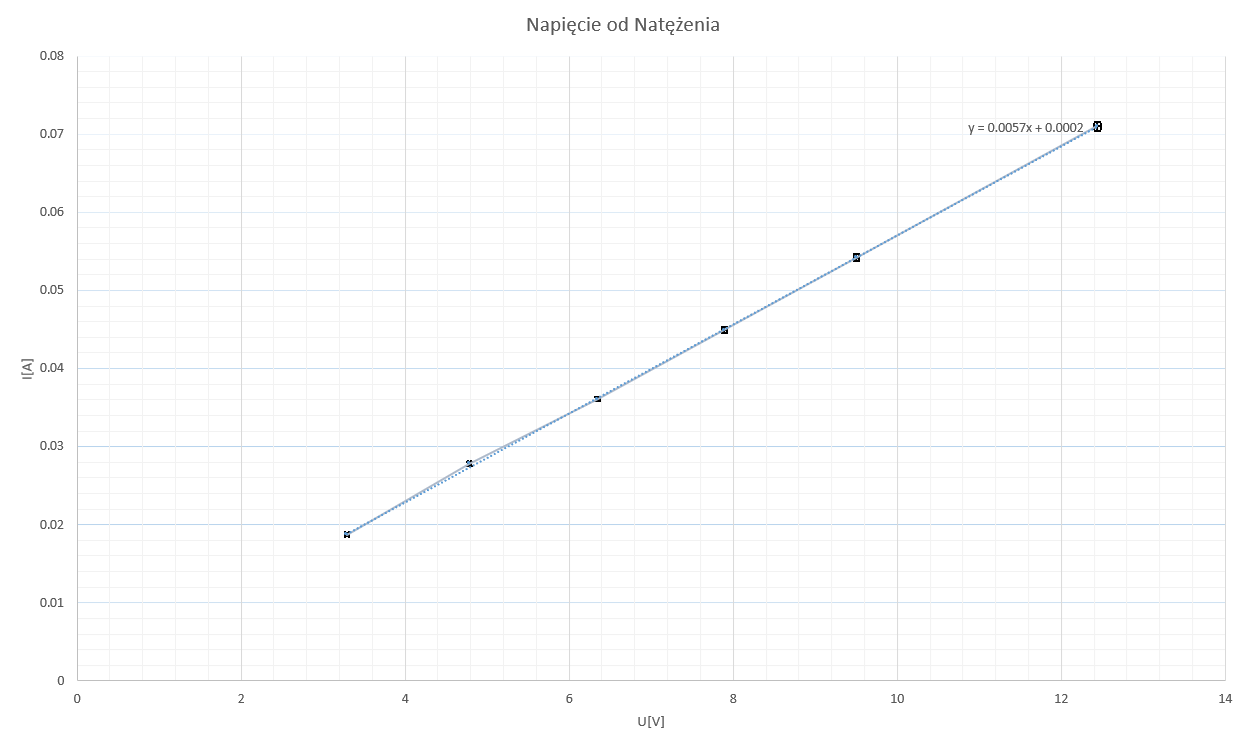
\includegraphics[width=\textwidth]{graph2.png}
    \caption{Wykres Napięcia od Natężenia z naniesionymi pomiarami, niepewnościami
     oraz linią trendu}
    \label{fig:mesh1}
\end{figure}
Wnioski:\\
Wyniki pomiarów przedstawione w tabeli z wynikami oraz na powyższym wykresie 
wyraźnie potwierdzają Prawo Ohma. Wszelkie niepewności pomiarowe są małe i 
nieznacznie wpływają na wynik pomiarów. 
\end{document}
